The default \gls{pdf} for the event generation is NNPDF2.3. The PDF
uncertainties are obtained by computing reweighting the signal samples to any of
the following three PDF sets: NNPDF2.3LO, CT10LO and MMH2014LO and also varying
each PDF set by its own uncertainties. This results in a large number of values
for the signal event yield in the signal
region. \cref{fig:susy_pdfsysts} shows an example of the observed
variation in the event yield (y-axis) for the three PDF sets, each systematic
variation of each PDF set is represented by a different position on the the
x-axis. The PDF systematic uncertainty is decomposed in:
\begin{itemize}
\item An uncertainty $\Delta \sigma$ on the overall normalisation or cross
  section, given by the variation of the total number of signal events,
\item An uncertainty $\Delta A$ on the signal acceptance, which is defined by
  the ratio of number of signal events in a particular bin of the signal region,
  divided by the total number of signal events.
\end{itemize}
This decomposition is done since the ATLAS standard is to depict the uncertainty
on the overall normalization as an uncertainty on the expected limits, while the
uncertainty on acceptance is to be incorporated in the uncertainty on the
observed limits. \cref{tab:susy_pdfsysts} presents the relative PDF uncertainty
on $\Delta \sigma$ and $\Delta A$ in the different bins of the signal region,
for each of the squark masses considered in the analysis. The uncertainty on the
cross section is between 19 and 26\%, increasing at higher squark mass. The
uncertainty on the acceptance increases for higher squark masses and at higher
$\met$ bins. At low squark mass and in the low $\met$ bin the statistics is
reduced and the systematic error increases due to low Monte Carlo statistics.
\begin{figure}[hb]
\centering
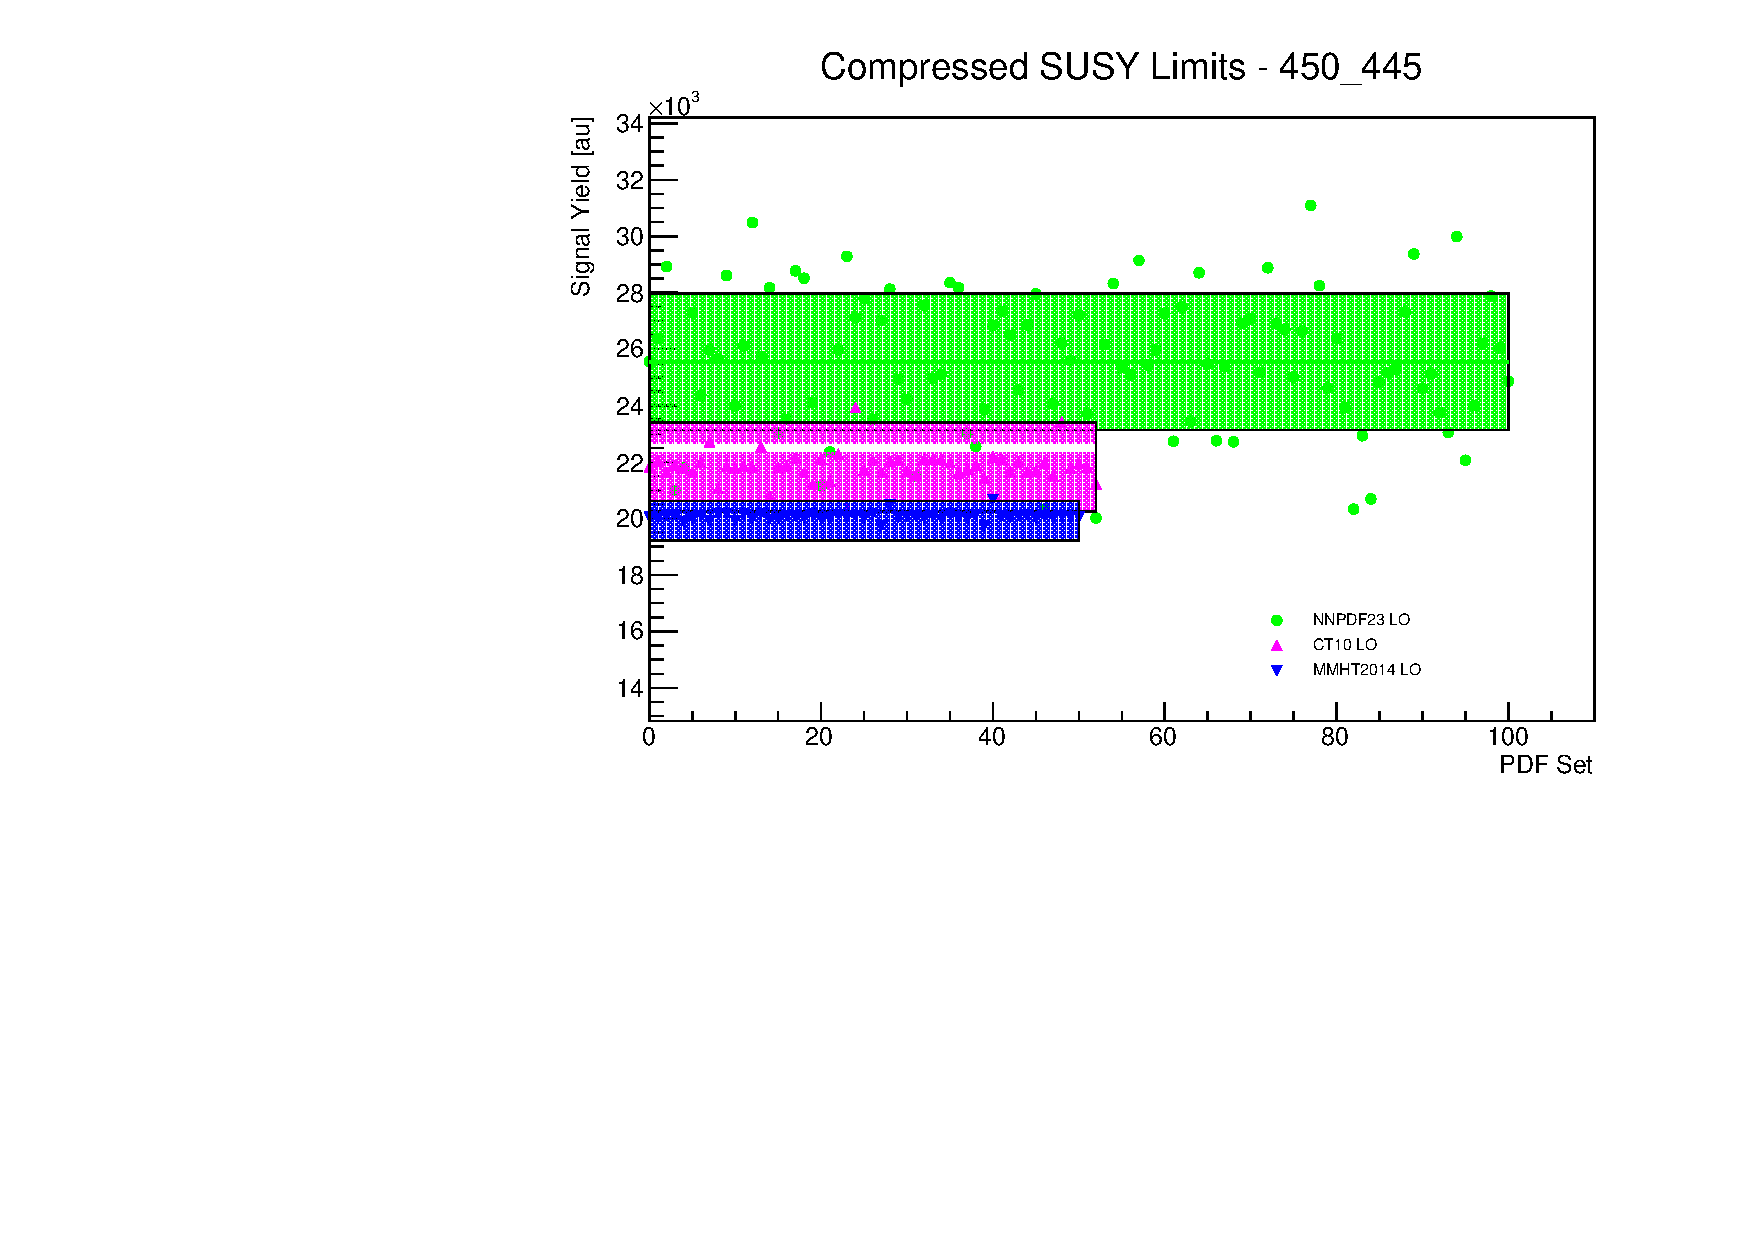
\includegraphics[width=0.9\linewidth]{450_445_MCut0_pdfset}
\caption{Variation in \gls{susy} compressed event yields for a model with
  $\msquark = 450$~GeV and $\mneutralino = 445$~GeV in the first $\met$ bin of
  the signal region ($250 < \met < 300$~GeV) for three \gls{pdf} sets
  NNPDF2.3LO, CT10LO and MMH2014LO. The $x$-axis represents the different
  systematic uncertainties associated to each \gls{pdf} set.}
\label{fig:susy_pdfsysts}
\end{figure}
\begin{table}
\centering
\small
\resizebox{\linewidth}{!}{\begin{tabular}{lccccccc}
  \toprule
  \multicolumn{8}{c}{\gls{pdf} Uncertainty} \\
  \midrule \midrule
  $\msquark$, $\mneutralino$ [GeV] &  400, 395 &
  450, 445 &  500, 495 &  550, 545 &  600, 595 &  650, 645 &  700, 695 \\
  \midrule
  $\Delta \sigma$  & 19 & 20 & 21 & 22 & 24 & 25 & 26 \\
  \midrule
  $\Delta A$ (250 $< \met <$ 300)  & 25 & 26 & 7 & 6 & 7 & 5 & 7\\
  $\Delta A$ (300 $< \met <$ 350)  & 5 & 7 & 5 & 4 & 4 & 4 & 4\\
  $\Delta A$ (350 $< \met <$ 400)  & 4 & 4 & 5 & 9 & 3 & 6 & 2\\
  $\Delta A$ (400 $< \met <$ 500)  & 6 & 2 & 6 & 5 & 2 & 7 & 9\\
  $\Delta A$ (500 $< \met <$ 600)  & 7 & 9 & 9 & 10 & 10 & 8 & 10\\
  $\Delta A$ (600 $< \met <$ 700)  & 8 & 10 & 6 & 14 & 13 & 10 & 9\\
  $\Delta A$ (700 $< \met$ )       & 10 & 9 & 16 & 15 & 17 & 16 & 14\\
  \bottomrule
\end{tabular}}
\caption{\gls{pdf} systematic uncertainties in \% on the SUSY compressed
  models. The uncertainty is the envelop that contains the signal yields from
  the three \gls{pdf} families, and their error bands. The first row indicates
  the systematic uncertainty on the overall normalisation. The following rows
  show uncertainty on the acceptance in the signal region $\met$ bins.}
\label{tab:susy_pdfsysts}
\end{table}
%%% Local Variables:
%%% mode: latex
%%% TeX-master: "../search_for_DM_LED_with_ATLAS"
%%% End:
